\documentclass[svgnames,final]{beamer}
\usepackage{etex}
\usepackage{multirow}
\mode<presentation> {
    \usetheme{I6dv}
}
\usepackage[utf8]{inputenc}
\usepackage[T1]{fontenc}
\usepackage[english]{babel}
\usepackage{amsmath,amsfonts,amsthm}
\usepackage{mathtools}
\usepackage{lmodern}
\usepackage{booktabs}
\usepackage[orientation=landscape,size=a0,scale=1.4]{beamerposter}
\usepackage{pgfplots}
\pgfplotsset{compat=1.9}
\usepackage{tikz}
\usetikzlibrary{positioning,plotmarks,calc,arrows,decorations.markings,intersections,backgrounds}
\usepackage{graphicx}
% \usepackage{xypic}
\usepackage{xy}
\usepackage{subfigure}
\graphicspath{{./images/}}

\newcommand{\normal}{\mathcal{N}}
\newcommand{\muhat}{\widehat{\mu}}

\newcommand{\red}[1]{\textcolor{red}{#1}}
\newcommand{\green}[1]{\textcolor{Green}{#1}}
\newcommand{\blue}[1]{\textcolor{blue}{#1}}
\newcommand{\ve}{\varepsilon}
\newcommand{\eps}{\ve}
\newcommand{\Otilde}{\widetilde{O}}
\newcommand{\poly}{\mathrm{poly}}
\newcommand{\dtv}{d_{\mathrm{TV}}}
\newcommand{\thres}{\mathrm{Thres}}
\newcommand{\tail}{\mathrm{Tail}}
\newcommand{\hood}{\mathcal{S}}
\newcommand{\E}{\mathbb{E}}

\DeclareMathOperator*{\argmin}{arg\,min}

\renewcommand{\arraystretch}{1.4}
\newcommand{\calG}{\mathcal{G}}
\newcommand{\calD}{\mathcal{D}}
\newcommand{\R}{\mathbb{R}}
\newcommand{\TV}{\mathrm{TV}}
\newcommand{\I}{\mathbb{I}}

\newcommand{\tplr}[1]{\hspace{.8cm}#1\hspace{.8cm}}

\newcommand{\specialcell}[2][c]{%
  \begin{tabular}[#1]{@{}c@{}}#2\end{tabular}}


\title{EC528 - Performance Analysis of Secure Multi-Party Computations in the Cloud}
\author{Hasnain Rehman \href{mailto:hasnain@bu.edu}{(hasnain@bu.edu)} \and Pierre-Fran\c{c}ois Wolfe \href{mailto:pwolfe@bu.edu}{(pwolfe@bu.edu)} \and Samyak Jain \href{mailto:samyakj@bu.edu}{(samyakj@bu.edu)} \and Suli Hu \href{mailto:sulihu@bu.edu}{(sulihu@bu.edu)} \and Yufeng Lin \href{mailto:yflin@bu.edu}{(yflin@bu.edu)}}
\institute{\textit{Boston University, College of Engineering}}

\begin{document}
\addtobeamertemplate{headline}{}
{\begin{tikzpicture}[remember picture, overlay]
    \node [anchor=north east, inner sep=1cm, outer sep=1cm]  at (current page.north east)
    {
\includegraphics[height=5cm]{bu}};
  \end{tikzpicture}}

\begin{frame}
  \vspace{-.5cm}
  
  \begin{columns}[T]
    % Column 1
    \begin{column}{.3\linewidth}
      
      \begin{block}{\large \textbf{\begin{center}Multi-Party Computation (MPC)\end{center}}}
        \textbf{MPC Benefits:}
        \begin{itemize}
          \item Enables mutually agreed computation using joint data
          \item Maintains privacy of data provided by each party
          \item No trust required in a single third-party for computation
        \end{itemize}
        \textbf{Some MPC Application Examples:}
        \begin{itemize}
          \item Marketplace with anonymous bidding
          \item Analyze medical data from multiple sources (HIPAA compliant)
          \item Salary trends for demographics from pool of companies
        \end{itemize}
        \begin{center}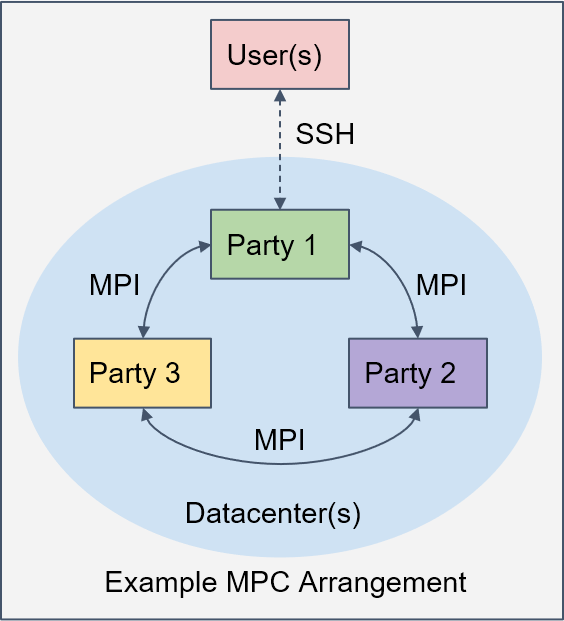
\includegraphics[width=0.75\textwidth]{three_party_overview.png}\end{center}
      \end{block}
      
      \begin{block}{\large \textbf{\begin{center} Project Goals\end{center}}}
        \textbf{Mentor Goals: (Already in progress at start of project)}
        \begin{itemize}
          \item Employ three-party Secret Sharing MPC
          \item Perform database queries across multiple private datasets
          \item Keep all operations secure vs. separating out insecure steps
          \item Implement clean MPC code with minimal dependencies
        \end{itemize}
        \textbf{Team Goals: (During Fall 2020 semester)}
        \begin{itemize}
          \item Deploy mentor MPC code on multiple platforms/configurations
          \item Improve benchmarking instrumentation for performance assessment
          \item Arrange a system of automation for easier ongoing testing
          \item Document and arrange information with an eye towards usability
        \end{itemize}
      \end{block}
      
    \end{column}
    
    % Column 2
    \begin{column}{.3\linewidth}
      
      \begin{block}{\large \textbf{\begin{center}Deployments Explored\end{center}}}
        \textbf{Why these Deployments?}
        \begin{itemize}
          \item Local and remote development environments
          \item Clients/data may or may not be co-located
          \item Performance/deployment difficulty tradeoffs
        \end{itemize}
        \textbf{Deployments}
        \begin{itemize}
          \item Local (Bare-Metal or virtualized)
          \item Cloud-based Virtual Machines (MOC OpenStack)
          \item Cloud-based Containers (MOC OpenShift)
          \item Bare-Metal Clusters (CloudLab)
        \end{itemize}
        \begin{table}
          \centering
          \begin{tabular}{ccc}
                           & LAN                                                & Ring                                                \\
            Single Cluster & 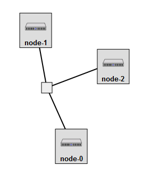
\includegraphics[width=.25\linewidth]{lan.png}     & 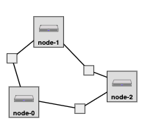
\includegraphics[width=.25\linewidth]{ring.png}     \\
            Multi Cluster  & 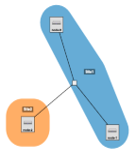
\includegraphics[width=.25\linewidth]{lan_geo.png} & 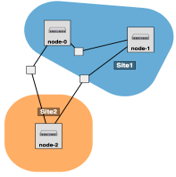
\includegraphics[width=.25\linewidth]{ring_geo.png} \\
          \end{tabular}
          \caption{CloudLab Topologies}
          \label{tab:cloudlab}
        \end{table}
      \end{block}
      
      \begin{block}{\large \textbf{\begin{center}Preliminary Results\end{center}}}
        \begin{center}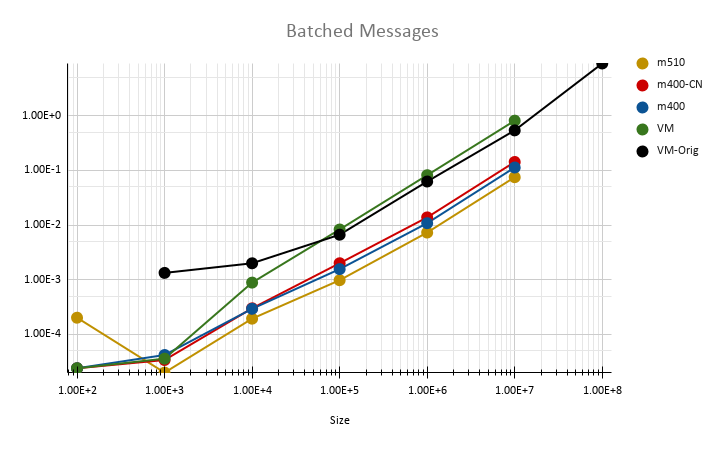
\includegraphics[width=\textwidth]{test_results.png}\end{center}
      \end{block}
    \end{column}
    
    % Column 3
    \begin{column}{.31\linewidth}
      
      \begin{block}{\large \textbf{\begin{center}Project Automation\end{center}}}
        \textbf{Features:}
        \begin{itemize}
          \item Easy to use and extend
          \item Leads to a repeatable end configuration state
          \item Simplifies both setup and testing
          \item Can support most/all desired scenarios
        \end{itemize}
        \textbf{Evolution:}
        \begin{enumerate}
          \item Manual installation, configuration, and testing
          \item Semi-automated: Shell scripts, geni-lib scripts, Dockerfiles, unpackable *.tar.gz,...
          \item Automated Software: Ansible package installation, system configuration, software build, test execution, data retrieval
        \end{enumerate}
      \end{block}
      
      \begin{block}{\large \textbf{\begin{center}Data Collection and Analysis\end{center}}}
        \begin{itemize}
          \item C code instrumentation with clock\_gettime
          \item Test input range and multiple samples output to *.csv
          \item Score-P wrapper for profiling MPI communication and more
          \item CUBE GUI for inspecting *.cubex and *.otf2 collections (below with execution tree expanded)
        \end{itemize}
        \begin{center}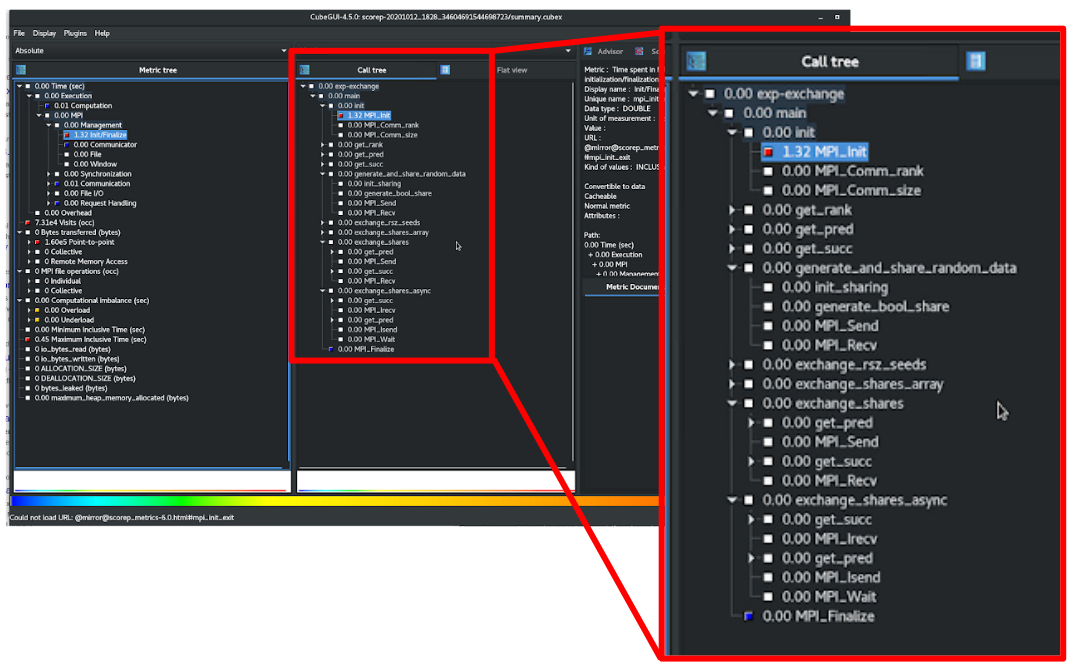
\includegraphics[width=\textwidth]{cube_gui.png}\end{center}
      \end{block}
      
      \begin{block}{\large \textbf{\begin{center}Future Work\end{center}}}
        \begin{itemize}
          \item Extend Ansible automation for additional OSs and environments
          \item Conduct additional MPI testing with tools developed
          \item Mentors wish to build a user frontend for deployment and testing
        \end{itemize}
      \end{block}
      
    \end{column}
  \end{columns}
\end{frame}
\end{document}
